\section{Model Class Implementations}
For various reasons described below, existing implementations of some models were not adequate for this research.
These reasons included speed, generality, and consistency.

\section{Model Execution: The Need for Speed}
Because optimization may involve an extremely large number of independent simulations of the same class of model, each varying only in model parameter values, it is critical that both the overhead for model instantiation and the duration of simulation itself, be as low as possible.
Existing modeling tools contain overhead associated with model initialization, shuttling results in memory, which are a trivial cost for single simulations, but begin to add up in optimization runs of thousands of simulations.  
Even the simulation of reduced models themselves are often slower than necessary using existing tools, due to some of these tools being written to accommodate more complex, biophysical models.
To overcome this and accelerate optimization, I built faster "pure python" implementations of two neuronal models (the Izhikevich model and the AdEx model).
One of the these was inspired from the existing MATLAB forward euler implementation of the Izhikevich model, while the other was adapted from an existing python implementation of the AdEx model using vectorized code.
While neither of these was especially fast, they provided the basic recipe upon which a faster Python implementation could be built.
Do note that the purpose of these new implementations was not model exploration, analysis, or sharing; existing tools are adequate for these purposes.
The purpose of the new implementations was simply to make large optimization runs computationally tractable.

Python does not have a reputation for speed; implementation details have a large impact on performance.
Therefore, I used a tool called \cite{numba} that enables Just-In-Time compilation (JIT) of Python code, making at fast as e.g. compiled C code.
This tool cannot be applied to any arbitrary Python code, so functions to which it is applied much be designed with only a subset of the usual syntax and library of Python.
In other words, it cannot be used to simply speed up any pre-existing Python code.
I hand-coded the two models above to be JIT-compliant, with the result that both became significantly faster than analogous models using NEURON or Brian2 simulators.
Importantly, simulation outputs retained a binary near-match in all cases, confirming that nothing was lost in the course of gaining this performance improvement.
I used these new implementations extensively throughout the project, and they are available to others at \href{https://github.com/russelljjarvis/IzhikevichModel} and XXXX.
The code that implements them is fairly easy to understand, share, and execute, and I hope they may be useful to others who have similar performance needs, either for optimization contexts or large network models where small performance gains are worth chasing.

\subsection{Model Design: Lack of Generality}
Significant time was spent in the early years of this project shoe-horning pre-existing tools into the desired optimization framework, with limited success.
These tools included, among others, model designers and neural simulators such as PyNN, Brian2, NEURON, and jNeuroML.
However, several unexpected road blocks were encountered on the way.

The \emph{NEURON} implementation of the Izhikevich model is fractured.
There are different implementations for different parameter regimes.
For a single simulation, this is not much of a problem.
However, it means that switching between such regimes during optimization (as would occur when a parameter value crossed a regime boundary), is a non-trivial exercise.
Even if successful, any source code successfully implementing this would be complicated, unreadable, and lack generality.
Specifically, NEURON requires NMODL files to be compiled for each different regime, and it may be difficult to know in advance which regimes the optimizer is likely to sample from.
Thus, the claimed performance of the C-based NEURON library is not actualized in an optimization context.
Because NEURON is well-understood within OSB and NeuroML community, I still used it only to produce reference simulations to verify that the output of my model implementations were in fact accurate.

PyNN provides the convenience of working in Python, and with a convenient procedural interface for model design and execution.
However, its implementations of most reduced models (e.g. Izhikevich) are simply "wrapped" versions of NEURON models; consequently PyNN has the same disadvantages as NEURON.
PyNN is also designed with network simulations in mind, which means its designers have chosen performance trade-offs that favor network simulations over single neuron simulations.
For example, a data-type called the "lazy-array" is the most elemental container for neuron models in PyNN, but it is meant to store populations of neurons as opposed to single neurons;
as such the lazy-array results in slow single neuron simulations \url{https://github.com/NeuralEnsemble/PyNN/issues/370}, \url{https://github.com/NeuralEnsemble/PyNN/issues/266}, which optimization depends on.
% The above links should be turned into citations.

A constant error warning plagued brian2 investmentallations was.
\begin{verbatim}
Brian2 causes error:
 ERROR      Brian 2 encountered an unexpected error. If you think this is bug in Brian 2, please report this issue either to the mailing list at <http://groups.google.com/group/brian-development/>, or to the issue tracker at <https://github.com/brian-team/brian2/issues>. Please include this file with debug information in your report: /tmp/brian_debug_t0acbm4l.log  Additionally, you can also include a copy of the script that was run, available at: /tmp/brian_script_juzhsbph.py Thanks! [brian2]
Traceback (most recent call last):
\end{verbatim}

To make optimization of models tractable it was important to do ongoing feasibility testing. For example its important to evaluate the the utility of established model implementations, as using these models to optimize may not in fact be feasible.\\ 
\\
Despite an a large number of choices of FOSS reduced model
implementations, many off the shelf implementations were not useful, or significant intervention was required to make some established implementations workable inside an optimization framework. \\
\\
In two classes of model a feasible choice of implementation did not exist and it was easier to re-implement those models. The two models I re-implemented were
the Adaptive Exponential Integrate and fire Model, and also the IZHI
model.  In the work below, I profile existing model implementations, and
justify the reasons for re-implementing.\\
\\
This is in contrast to the brian2/neuraldynamics AdExp model, which took
between 2 or 3 times longer to find a rheobase current injection value. However the slowness is not caused by the simulation backend (brian2 which is relatively fast and efficient). The slow down is caused by the way the model is defined. Specifically the
model is defined in a middle code layer neurodynamics\cite{gerstner2014neuronal}.\\
\\
It is very likely, that the model implementation is correct, since Gerstner is an author of one of the original adaptive exponential publications, and the neural dynamics book that the brian2 code is strongly affiliated with. Since Integrate and Fire models don't formally include spikes when an implementation does include spikes, it is an optional add on.\\
\\
The AdExp neurodynamics models default implementation causes spikes with peaks below $0mV$, since the IZHI model like all integrate and fire models do not explicitly include spikes\\
\\
This is not technically wrong, but it violates
assumptions in the \emph{NeuronUnit} feature extraction protocol. The default spiking behavior, looks odd, and it is simply this poor model definition that is causing a slower optimizer performance. The optimizer takes an unusual waveform shape, and searches for longer in distant
parameter regions to find a good fit.\\
\\
Over the course of evaluating the brian neural dynamics model \cite{gerstner2014neuronal}. I experienced some phenomena that only occurred in the context of genetic algorithm optimization. The reason why optimization provides a different evaluation context is because, in optimization simulation objects are required to be created and destroyed rapidly and on mass. Brian2 is designed to be an efficient network simulator, the case of being designed for network simulation, may assume you will want to create a lot of neural models that persist efficiently together in memory (this was also a problem with PyNN models). Therefore you might see below, that while only one brian model exists in memory, performance is okay, but when creating and destroying models rapidly and on mass a slow down occurs.\\
\\
Below I have implemented a python integrator for the Adaptive
Exponential Integrate and fire model. This solver lead to faster
evaluations of current injection experiments. The integrator I developed
had a $0mV$ spiked when evaluated at default
parameter values.\\


Brian2 and sciunits sometimes collided in name space, and logging.
%\href{https://github.com/scidash/sciunit/pull/124/files/83907ba68740642178ebb91084f6e382e06a43c4#diff-d68791d2ed5dfaa96a900be6180bd950}

\section{Profiling the JIT enabled AdExp Model}
Mean time taken on single model evaluation:$ 0.0012554397583007812s $
Mean time taken to compute Rheobase:
$0.183s $
This was slightly faster than Izhikevich implementation which was for total rheobase solution $ 0.462s $ and $  0.002 s$ per run. Solving for Rheobase takes a average of 15 model evaluations.
%\begin{figure}    
%\begin{center}
%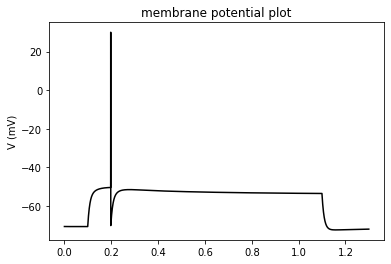
\includegraphics[width=0.25\linewidth]{figures/backend_check_files/backend_check_6_2.png}
%\caption{}

%\end{center}
%\end{figure}

%\begin{verbatim}
%    251 ms +- 5.02 ms per loop (mean +- std. dev. of 2 runs, 1 loop each)
%    240 ms +- 11.1 ms per loop (mean +- std. dev. of 2 runs, 1 loop each)
%    223 ms +- 12.5 ms per loop (mean +- std. dev. of 2 runs, 1 loop each)
%\end{verbatim}

\begin{verbatim}
    922 ms +- 12.7 ms per loop (mean +- std. dev. of 7 runs, 1 loop each)
\end{verbatim}

\subsection{Compare parallel to serial speeds, and accuracy}

Below is the Brian2/NeuralDynamics AdExp model. In-order to make the spike height greater than $0mV$ it was easier to use computer code to schedule waveform modifications that occur straight after the the brian2 simulation, these scheduled waveform modifications can be considered part of a peripheral shell of simulation code. In postprocessing
the waveform data type is a Neo Wave form object that is artificially the algorithm of determining rheobase and displaying results. The time of this model is determined on multiple factors, as discussed elsewhere, execution time is not uniform across model parameterizations. Models with multispiking behavior will take longer to solve.

Simulation times for this model vary, dramatically possibly because of
lazy evaluation, the simulation times may vary according to what else
you are running on your computer. Not all models experience a speed up when executed in parallel, however
this model was faster in the parallel Rheobase determination algorithm. Some common times are: $3.92,6.75,4.48,5.17$. Mean time was:

\subsection{Comparison of Times Taken to Find Rheobase}
Custom implementation JIT enabled implementation: $4.0s$. 
Brian2 taken to find Rheobase: $4.40s$ (serial), $3.976s$ (parallel).

The evaluation times between Brian2 and the custom written
integrator are similar. Both have average rheobase solution times of approximately 4 seconds, however the spike shape derived from the custom written integrator look more realistic under default paramaterizations. The biological plausibility of default model paramaterization has consequences for model optimization speed, because when  models undergo mutation and cross-over the mean of random models regressors towards the default model initialization, and if the default model is a bad fit to data, the average model sampled by the genetic algorithm will also be bad to data.\\

\begin{figure}
\begin{center}
\centering
  \centering
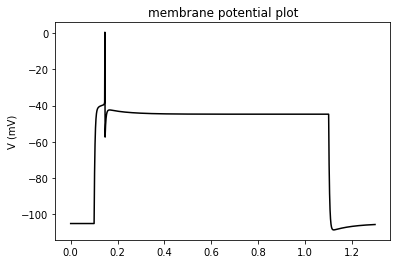
\includegraphics[scale=0.45]{figures/backend_check_files/backend_check_12_10}
\caption{Model parameterization of the brian2 simulator with the customization: interpolated spike height, forced to be above $0mV$}

  \label{fig:sub1}
  \centering
  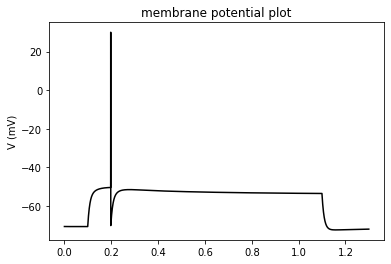
\includegraphics[scale=0.45]{figures/backend_check_files/backend_check_4_2}
    \caption{Default model parameterization of the custom written integrator}
  \label{fig:sub2}
\caption{Comparison between two Adxaptive Exponential Implementations}
\label{fig:test}
\end{center}
\end{figure}




    
$272 ms +- 66.5 $/mu$s per loop (mean +- std. dev. of 2 runs, 1$ loop each)

The next model to be evaluated is the NEURON Izhi model. The NEURON Izhi model has various draw backs. 1. It depends on an external file which must be recompiled each time this project is recreated. 2. The build environment of NEURON is non-trivial, and only a super dedicated NEURON modeller would install it on their system. Any performance advantage of using NEURON investment does not exceed the installation cost of installing the program. 3. The model implementation code is less generalizable than than the published Izhi model itself. Where the standard NEURON-NeuroML code only covers the Regular-Spiking model * This is likely due to a name space conflict between Capacitance. Neuron has a `capacitive' mechanism inside modelled Neurons, this particular model has section capacitance as well as an introduced capacitive term inside a C-compiled mechanism. Both contribute to a the membrane
potential calculation. * The NEURON Izhi model took $78$ seconds to find the rheobase current injection value $ 51.79367065 * pA $.

    
%\begin{center}
 %   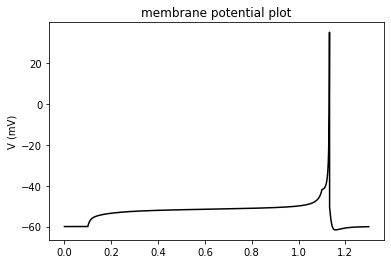
\includegraphics[width=0.7\textwidth,]{chapters/figures/backend_check_files/backend_check_14_2.png}
%    \caption{where is picture}
%\end{center}


%\begin{figure}
%    \centering
%    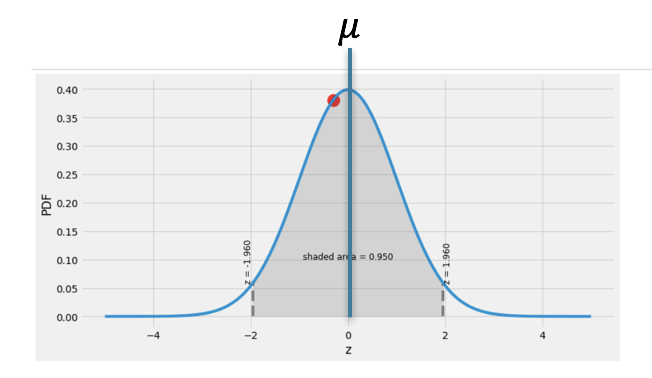
\includegraphics{chapters/normal_distribution}
%    \caption{This is your image%}
%    \label{fig:my_label}
%\end{figure}
%A tool numba JIT

% https://www.overleaf.com/learn/how-to/Images_not_showing_up 
        
The forward Euler python IZhi model is very fast. The forward euler
implementation utilized Numba JIT \cite{lam2015numba}. Rheobase is found in under a second,
and in many cases close 0.5 seconds. This represents a very dramatic
speed up. Unlike the NEURON NeuroML implementation of the izhikitich equation,
this implementation is just as generalizable as the original MATLAB
implementation of the izhikitich model.

%\begin{verbatim}
%  time taken on
%  block 0.6859951019287109 \textbackslash{}n3.3 ms +- 9.79 %$\mu$s per loop (mean +- std. dev. of 2
%  runs, 100 loops each)\textbackslash{}n3.32 ms +- 30.9 us per loop (mean +- std. dev. of 2 runs,
%  100 loops each)\textbackslash{}n3.19 ms +- 10.9 us per loop (mean +- std. dev. of 2 runs, 100
%\end{verbatim}
        
\section{Python/LEMS and NEURON versions of single compartment Conducance Model.}

Conductance based models took approximately the same amount of
time to evaluate the Rheobase search algorithm as the python
implementation.

%This problem in the default parameterization of the python model was later located in the scale or units of capacitance, if default capacitance parameterization is multiplied by 100.0 the problem goes away.

time taken to compute rheobase $ 12.6s $

%\begin{center}
%\includegraphics{figures/backend_check_files/backen%d_check_22_2}
%\end{center}

%$ 1.40762329 * pA $


\subsection{NEURON versions of single compartment Conducance
model.}

Hodgkin Huxley Conductance based channels models took approximately the same amount of time to evaluate the Rheobase search algorithm as the python implementation.

%The NEURON implementation was slightly faster, and the default parameterization of the model lacked `ringing'', or below threshold oscillations that the Python ODE version had under default conditions.

%This problem in the default parameterization of the python model was later located in the scale or units of capacitance, if default capacitance parameterization is multiplied by 100.0 the problem goes away.

    \begin{verbatim}
time taken on block 8.573923826217651
    \end{verbatim}

The author also engineered GLIF model support for $NeuronUnit$ tests. In practice these models where hard to configure without expert knowledge, GLIF models contain the most parameters of all models, and many of these parameters are vectors, not scalars. GLIF models do not visualy spike which makes debugging their behavior very difficult. None the less GLIF models where among the fastest to evaluate, and the author had success in making fitting these models to Allen Rheobase data.

    %\graphicspath{ {../figures/} }
%    \begin{center}
%    \begin{figure}
%    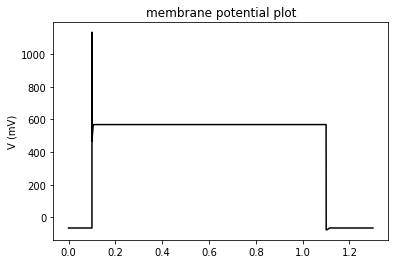
\includegraphics{figures/backend_check_files/backend_check_26_2}
    %kend_check_files/backend_check_26_2.png}
%    \end{figure}
    
%    \end{center}
%\begin{verbatim}
% 112.5 pA
%'value': array(1.40645904) * pA
%\end{verbatim}

% parameters of an adaptive exponential model
%\begin{verbatim}
%\{'El\_reference': -0.07016548013687134, %'C': 3.990452661875942e-10%,
%'init\_threshold': 0.02964956889477108, %'th\_inf': 0.02964956889477108,
%'spike\_cut\_length': 109.5, %'init\_voltage': -35.0, 'R\_input': %910258965.9792937\}
%\end{verbatim}
$ Rheobase = 112.5pA $

time taken to execute this model.
$ 0.23476457595825195 $

    


%$ 112.5 pA $
%$0.0 mV$ $-0.065 mV$

%    \begin{verbatim}
%    \{'value': array(183.33333333) * pA\}
%    \end{verbatim}

%\begin{verbatim}
%array(112.5) * pA
%\end{verbatim}


%\begin{verbatim}
%    0.017240506310425608 mV -0.08583939747094235 mV
%    0.017240506310425608 mV% -0.08583939747094235 mV
%\end{verbatim}

    %\begin{center}
    %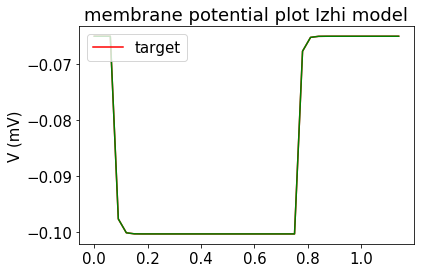
\includegraphics{figures/backend_check%_files/backend_check_32_2.png}
    %\end{center}
